% !TEX encoding = IsoLatin2  % notwendige Zeile f"ur Mac-Benutzer (muss als Kommentar stehen); Windows-Benutzer k"onnen
%die Zeile l"oschen.

% LaTeX-Vorlage Version 3.1,  Juli 2011
% erstellt von Dr. Andreas Drauschke (andreas.drauschke@technikum-wien.at) und Dr. Susanne Teschl (susanne.teschl@technikum-wien.at)
% geringf"ugig adaptiert von Harald Stockinger (harald.stockinger@technikum-wien.at)


\documentclass[11pt,a4paper,bibtotoc,oneside]{scrbook}
% F"ur kurze Arbeiten w"are auch die Dokumentklasse "scrartcl" ausreichend. In diesem Fall ist "section" die h"ochste Ebene ("chapter" gibt es dann nicht).
% \documentclass[a4paper,bibtotoc,oneside]{scrartcl}


%Zum Verlinken des inhaltsverzeichniss & co
\usepackage[colorlinks=false]{hyperref}
% %hyperref setup`%
\hypersetup{pdfborder=0 0 0}
%       colorlinks=false,
%       citecolor=Violet,
% %         linkcolor=Green}
\usepackage[utf8x]{inputenc}
% deutsche Anpassungen
% \usepackage[ansinew]{inputenc}
\usepackage[T1]{fontenc}
\usepackage[ngerman]{babel}
% mathematische Symbole
\usepackage{amsmath,amssymb,amsfonts,amstext}
\usepackage{xcolor}
\usepackage{calc}
\usepackage{caption}
%tabellen

% Kopfzeilen frei gestaltbar
\usepackage{fancyhdr}
\lfoot[\fancyplain{asdf}{}]{\fancyplain{}{}}
\rfoot[\fancyplain{}{}]{\fancyplain{}{}}
\cfoot[\fancyplain{}{\footnotesize\thepage}]{\fancyplain{}{\footnotesize\thepage}}
\lhead[\fancyplain{}{\footnotesize\nouppercase\leftmark}]{\fancyplain{}{}}
\chead{}
\rhead[\fancyplain{}{}]{\fancyplain{}{\footnotesize\nouppercase\sc\leftmark}}

% Farben im Dokument m"oglich
\usepackage{color}

% Schriftart Helvetica
\usepackage{helvet}
\renewcommand{\familydefault}{cmss}

% Graphiken einbinden: hier f"ur pdflatex
\usepackage[pdftex]{graphicx}
% Um pdf einzufügen
\usepackage{pdfpages}
\usepackage{array}

% H"ohe und Breite des Textk"orpers etwas gr"osser definieren
\setlength{\textheight}{260mm}
\setlength{\textwidth}{1.05\textwidth}

% weniger Warnungen wegen "uberf"ullter Boxen
\tolerance = 9999
\sloppy

% Anpassung einiger "Uberschriften
\renewcommand\figurename{Abbildung}
\renewcommand\tablename{Tabelle}

% %footers and headers
% % \usepackage{fancyhdr}
% % \pagestyle{fancy}
% \lhead{\studiumshort}
% \chead{}
% \rhead{\fachnameshort}
% \lfoot{\teilnehmeronenachname, \teilnehmertwonachname}
% % \cfoot{erstellt am: \today}
% \rfoot{\thepage}
% \renewcommand{\headrulewidth}{0.5pt}
% \renewcommand{\footrulewidth}{0.5pt}
\usepackage{geometry}
\begin{document}
% Kopf- und Fusszeilen initiieren
\pagestyle{fancy}

% Deckblatt:
\thispagestyle{empty}
\begin{picture}(0,0)
\color{white}\sffamily
\put(-101,-390){
\includegraphics[width=1.002\paperwidth]{./picture/LPS_2011.pdf}}
\put(220,-670){
\includegraphics[width=0.5\textwidth]{./picture/FHTW_Logo_4c.pdf}}
\put(-30, -20){\bfseries\huge SEMINARARBEIT}
% Titel des Studienganges einf"ugen:
\put(-30,-50){\Large im Studiengang BEL3}
% Titel der Lehrveranstaltung einf"ugen:
\put(-30,-70){\Large Lehrveranstaltung Audiotechnik}
\color{black}
% Titel der Arbeit einf"ugen:
% Die Minipage wird gesetzt, damit auch mehrzeilige Titel m"oglich werden.
\put(-32,-350){
\begin{minipage}{13cm}
\bfseries\huge D-Verstärker
\end{minipage}
}
% Name der Autorin/des Autors eingeben:
% Personenkennzeichen der Autorin/des Autors eingeben:
\put(-30,-450){\large Ausgeführt von:\ Christian Schwarzgruber}
\put(+54,-470){\large \ Alexander Rössler}
\put(-30,-490){\large Matrikelnummer: 1110254027}
\put(+63,-510){\large 1110254020}
% Name der Begutachterin/des Begutachters eingeben:
\put(-30,-550){\large Begutachter: Michael Windisch}
\put(-30,-590){\large Wien, \today} % das Datum des letzten Kompilierens wird automatisch eingesetzt
\end{picture}

<<<<<<< HEAD
=======
wieder löschen blalalal
>>>>>>> 2c0cc00f792935d39450d32db81a91301a5f800f
\savegeometry{GEO1}
\newpage

\tableofcontents\thispagestyle{empty}
\newpage

\setcounter{page}{1}
\newgeometry{top=25mm, left=25mm, right=25mm, bottom=25mm, headsep=2mm, footskip=2mm}
\savegeometry{GEO2}
% Falls die Kapitel"uberschriften zu lang f"ur die Kopfzeile oder das Inhaltsverzeichnis sind, so erzielt man
% dort Kurzformen der Kapitelbezeichnungen mittels:
% \chapter[Kurzform]{Lange "Uberschrift}
\chapter[Recherche über Klasse D-Verstärker]{Recherche über Klasse D-Verstärker}

%=====================================================================================================================%
\section{Recherche}
Es gibt unzählige Möglichkeiten einen Klasse D-Verstärker zu
implementieren, doch besitzen sie allesamt die selben
Grundbauelemente, wie Schmiddtrigger und Dreiecksgenerator.\\ Oft wird eine analoge PWM-Steuerung verwendet um, dass
Signal mit nur zwei Spannungszuständen zu erzeugen. Es gibt noch verschiedene andere analoge und digitale Verfahren
bzw. Verfeinerungen, wie Pulsfrequenzmodulation, Simga-Modulation oder
Sliding-Mode-Regelung.\textcolor{blue}{\cite{digWik}}
Bei der Recherche sind wir auf eine gute Anleitung gestoßen, die auch noch dazu sehr gut erklärt
ist.\textcolor{blue}{\cite{cae}}
Im Internet findet man unzählige Anleitungen über den Aufbau von Klasse-D-Verstärker, manche sind sehr umfangreich und
detailliert erklärt.
\section{Funktionsweise}
Das eingangs Signal wird zunächst in ein Digitales Signal umgewandelt, meist geschieht das mit einer PWM-Steuerung, wie
oben beschrieben. Dieses Signal ist ist nun viel Hochfrequenter und kann so Verlustarm verstärkt werden. Die PWM kennt
nur zwei Zustände 1 und 0, sprich High und Low.
\section{Verwendungsmöglichkeiten von Klasse D-Verstärker}

\section{Alternativen}
\subsection{A-Verstärker}
Klasse ``A-Verstärker'' besteht aus einer Transistor Schaltung mit einem Transistor. Der Arbeitspunkt liegt
in der Mitte. Diese Klasse wird heute kaum noch verwendet Grund hierfür ist der geringe
Wirkungsgrad von nur 6.25\%, unabhängig von der Last. Das heißt wenn ein Verstärker der Klasse-A ein Ausgangsleistung
von 10 Watt liefert wandelt es ständig 60 Watt in Wärmeenergie um. \textcolor{blue}{\cite{csA}}
\subsection{B-Verstärker}
Beim Klasse B-Verstärker werden mindestens zwei Transistoren verwendet. Geht man von einem Sinus Signal aus, leitet der
eine Transistor bei der Positiven Halbwelle während der andere Transistor sperrt, somit nimmt der zweite Transistor
keine  Leistung auf. Bei negativer Halbwelle leitet der Transistor zwei während der Transistor eins Sperrt.
Nachteil ist das bei einer Eingangsspannung nahe dem Nullpunkt keine Übertragung stattfindet, aufgrund der
Basis-Emitter Dioden.
Der Wirkungsgrad liegt beim Klasse-B-Verstärker bei 70\%.
\textcolor{blue}{\cite{csA}}
\subsection{AB-Verstärker}
Der Klasse-AB-Verstärker ist eine Kombination aus Klasse A und B. Bei dem Klasse-AB-Verstärker werden wieder mindestens
zwei Transistoren verwendet. Durch weitere Erweiterung der Schaltung fließt ein Ruhestrom, der dafür sorgt die
Verzerrungen während des wechseln von der Negativen zur Positiven Halbwelle zu linearisieren.
Der praktische Wirkungsgrad liegt weiterhin bei 70\%.
\textcolor{blue}{\cite{csA}}
\subsection{Weitere Verstärker}
\begin{itemize}
    \item E-Verstärker
    \item    H-Verstärker
\end{itemize}

\textcolor{blue}{\cite{csA}}
%=====================================================================================================================%
\chapter[Dreiecksgenerator, Komperatorschaltung und Treiberstufe]{Bauteile}
\section{Dreiecksgenerator}
\subsection{Schaltungsaufbau}
    \begin{figure}[ht]
    \centering
        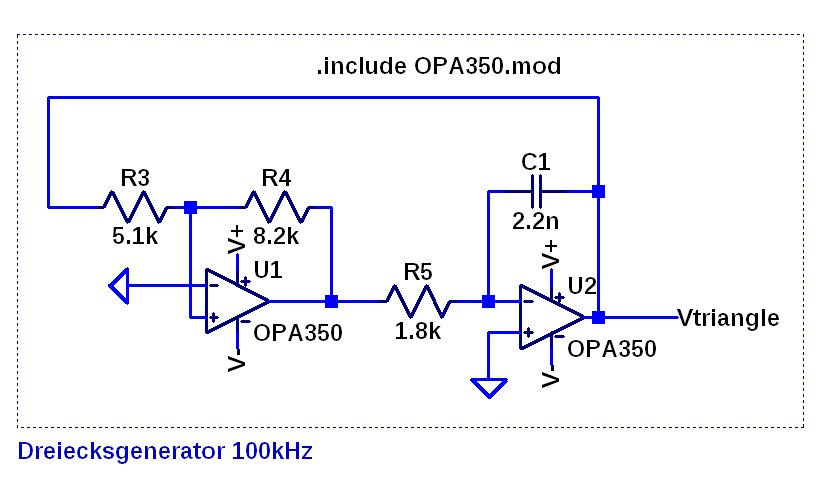
\includegraphics[width=300pt]{./picture/dreiecksgenerator.png}
        % LM324_triangle.png: 0x0 pixel, 250dpi, 0.00x0.00 cm, bb=
        \caption{\label{lm324}{Dreiecksgenerator}}
    \end{figure}
\subsection{Dimensionierung}
Irgentwie. -> lol :-)
\subsection{Funktionsweise}
\newpage
\section{Komperatorschaltung}
\subsection{Schaltungsaufbau}
    \begin{figure}[ht]
    \centering
        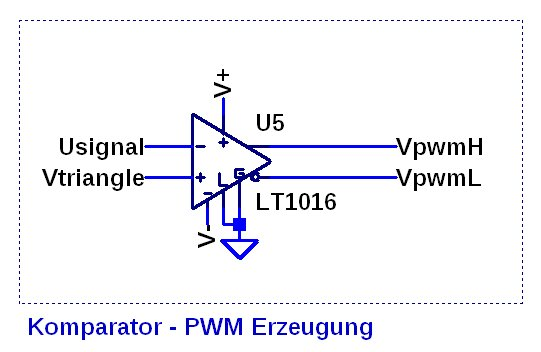
\includegraphics[width=300pt]{./picture/pwm.png}
        % LM324_triangle.png: 0x0 pixel, 250dpi, 0.00x0.00 cm, bb=
        \caption{\label{lm324}{PWM Erzeugung durch Komparator}}
    \end{figure}
\subsection{Dimensionierung}
\subsection{Funktionsweise}
% \newpage
\section{Treiberschaltung}
\subsection{Schaltungsaufbau}
    \begin{figure}[ht]
    \centering
        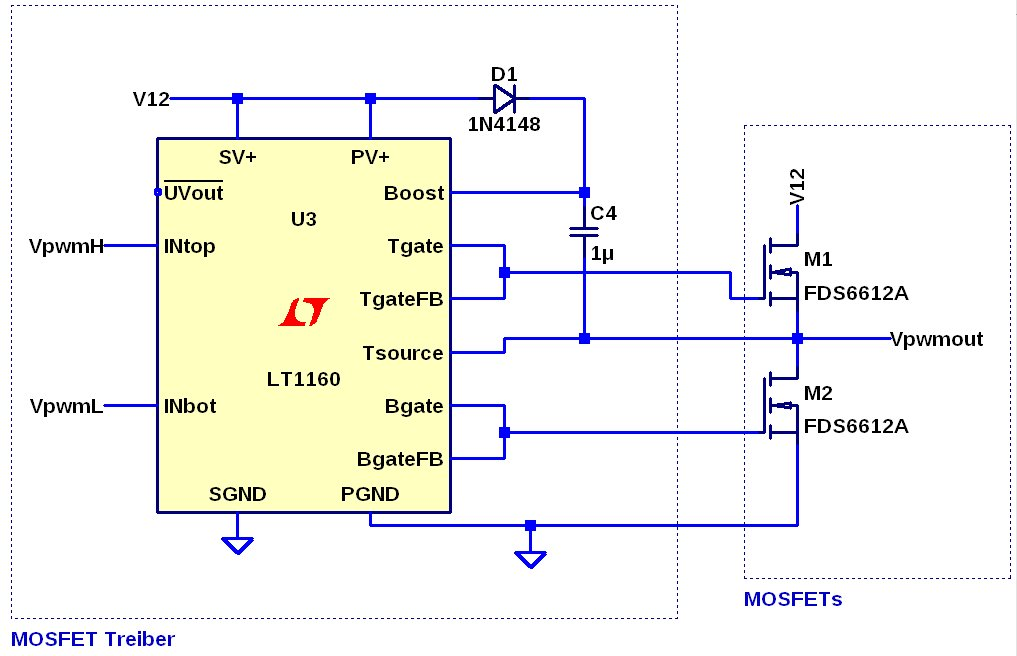
\includegraphics[width=300pt]{./picture/treiber.png}
        % LM324_triangle.png: 0x0 pixel, 250dpi, 0.00x0.00 cm, bb=
        \caption{\label{lm324}{MOSFET Treiber}}
    \end{figure}
\newpage
\subsection{Dimensionierung}
    \begin{figure}[ht]
    \centering
        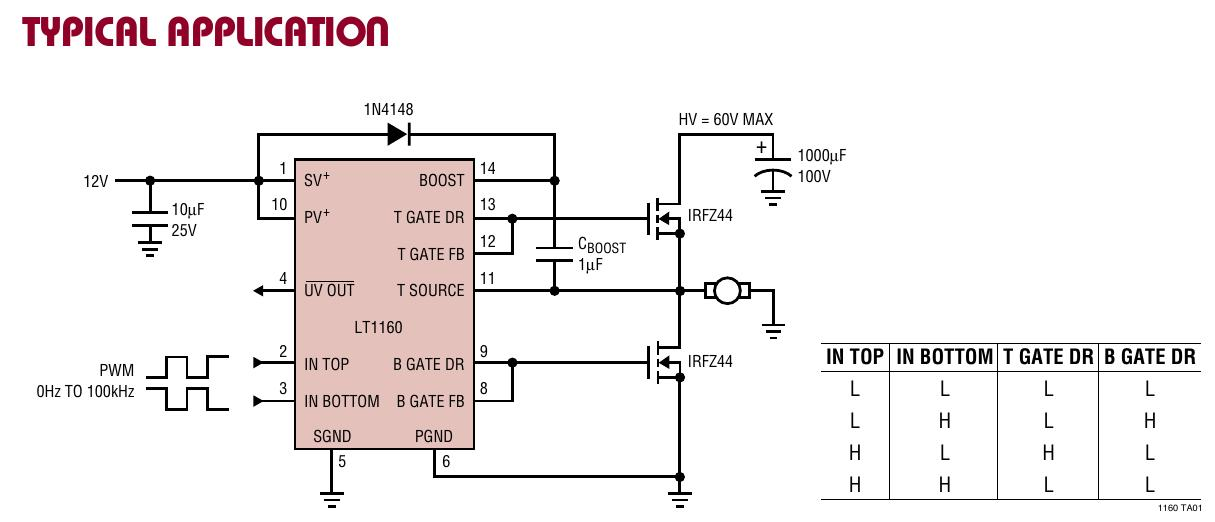
\includegraphics[width=300pt]{./picture/treiber_orig.png}
        % LM324_triangle.png: 0x0 pixel, 250dpi, 0.00x0.00 cm, bb=
        \caption{\label{lm324}{Treiberschaltung laut LT1160 Datenblatt}}
    \end{figure}
\subsection{Funktionsweise}

\chapter{OPV Vergleich}
\section{OPV-LM324}
Der OPV-LM324 hat eine sehr geringe Slew Rate von nur 0.5 $V/µs$ dies ist der Grund warum das Ausgangssignal nicht dem
Eingangssignal folgen kann. Siehe Abbildung \textcolor{blue}{\ref{lm324}}
\subsection{Simulation}
    \begin{figure}[h]
    \centering
        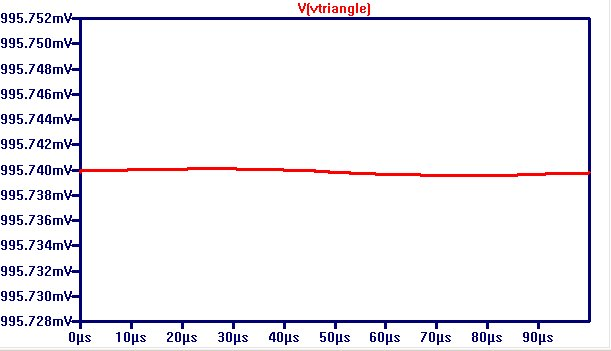
\includegraphics[width=300pt]{./picture/LM324_triangle.png}
        % LM324_triangle.png: 0x0 pixel, 250dpi, 0.00x0.00 cm, bb=
        \caption{\label{lm324}{Ausgangssignal LM324}}
    \end{figure}
    % LM324_triangle.png: 0x0 pixel, 250dpi, 0.00x0.00 cm, bb=
\section{OPV-OPA350}
Der OPV-OPA350 hat eine sehr hohe Slew Rate von 22 $V/µs$ welche sich bemerkbar macht. Das Ausgangssignal kann dem
Eingangssignal folgen. Siehe Abbildung \textcolor{blue}{\ref{opa324}}
\subsection{Simulation}
\begin{figure}[h]
\centering
    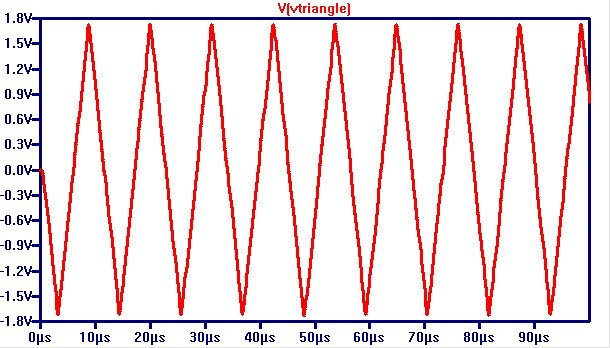
\includegraphics[width=300pt]{./picture/OPA350_triangle.png}
    % OPA350_triangle.png: 0x0 pixel, 250dpi, 0.00x0.00 cm, bb=
    \caption{\label{opa324}Ausgangssignal OPA350}
\end{figure}
\chapter{Klasse-D-Verstärker Schaltung}


\chapter{Seminarbuch}
\begin{table}[htbp]
  \centering
  \captionsetup{margin=1pt,font=small,labelfont=bf}
  \caption{Tätigkeit}
    \begin{tabular}{| c | c| }\hline
    {\bf Arbeitstag} &{\bf Tätigkeit} \\\hline
    \hline
    1. Tag   & Recherche im Internet über D-Verstärker  \\
    2. Tag   & Dimensionierung der Dreiecksgenerators und Simulation \\
    3. Tag   & Durchführung Übung 3 Signalkennwerte Messung  \\
    4. Tag   & Durchführung Übung 3 Signalkennwerte Messung  \\
    4. Tag   & Durchführung Übung 3 Signalkennwerte Messung  \\
    \hline
    \end{tabular}%
  \label{tab:addlabel}%
\end{table}%
\begin{table}[htbp]
  \centering
    \captionsetup{margin=1pt,font=small,labelfont=bf}
      \caption{Arbeitsaufwand}
      \begin{tabular}{| c | c |}\hline
      {\bf Arbeitszeit(h)} &{\bf Dokumentation(h)} \\\hline
      \hline
        2   & 2 \\
        2   & 2 \\
        4   & 7 \\
      \hline
        \textbf{12}   & \textbf{14} \\
      \hline
      \end{tabular}%
    \label{tab:addlabel}%
\end{table}%






\restoregeometry

\bibliographystyle{IEEEtran}
\bibliography{Literatur}

% Abbildungsverzeichnis
% \listoffigures
% \addcontentsline{toc}{chapter}{Abbildungsverzeichnis} % f"ugt den Eintrag "Abbildungsverzeichnis" im Inhaltsverzeichnis hinzu
% % \newpage
%
% % Tabellenverzeichnis
% \listoftables
% \addcontentsline{toc}{chapter}{Tabellenverzeichnis} % f"ugt den Eintrag "Tabellenverzeichnis" im Inhaltsverzeichnis hinzu
% % \newpage

% Abk"urzungsverzeichnis
% Bei Verwendung der Dokumentklasse "scrartcl" ist der Befehlt \addchap{Abk"urzungsverzeichnis} durch
% \addsec{Abk"urzungsverzeichnis} zu ersetzen
\addchap{Abk"urzungsverzeichnis}
\hspace{-17mm}\begin{tabular}{>{\raggedleft}p{0.2\linewidth} p{0.75\linewidth} p{0.1\linewidth}}
PWM & Pulsweitenmodulation \\
URL & Uniform Resource Locator
\end{tabular}

% Anh"ange
% \begin{appendix}
% \chapter[Erster Anhang]{Entwicklung und Aufbau eines Klasse D-Verstärkers}
% % \lhead{}
% % \lhead{\textcolor{blue}{\url{www.widatec.com/}}}\label{Anhang1}
% % \includepdf[pages={1-24},addtotoc={{24},{section},{2},{Entwicklung und Aufbau eines Klasse
% % D-Verstärkers},{D-Verstärker}}, pagecommand={\thispagestyle{fancy}},noautoscale=true,width=1.1\textwidth,offset=0cm
% % 1cm]{/home/christian/FH/3.Semester/ATK/Projekt/seminararbeit1/unterlagen/CAE.pdf}
% % \lhead{\studiumshort}
% %
%
% \chapter[Zweiter Anhang]{"Uberschrift des zweiten Anhangs}
%
% Text Text Text Text Text Text Text Text Text Text Text Text Text Text Text Text Text Text Text Text Text Text Text Text ...
%
% \end{appendix}

\end{document}
